\documentclass[areasetadvanced]{scrartcl}

\usepackage[utf8]{inputenc}
\usepackage[T2A]{fontenc}
\usepackage[english,russian]{babel}

\usepackage[footskip=1cm,left=25mm, right=15mm, top=20mm, bottom=20mm]{geometry}
\usepackage{setspace}
\usepackage{amsmath, amssymb}  % Объединено в одну строку
\usepackage{graphicx}
\usepackage{booktabs,longtable}
\usepackage{tikz}
\usetikzlibrary{arrows.meta}
\usepackage{float}
\usepackage{dashrule}
\usepackage{fancyhdr} % оформление отчёта
\usepackage{hyperref} % оформление отчёта
\usepackage{parskip}
\usepackage[strings]{underscore}

\usepackage{textcomp, enumitem}
\usepackage{indentfirst}
\usepackage{graphicx}
\usepackage{algorithm}
\usepackage{algpseudocode}
\usepackage{array}  % Для использования команды m{}
\usepackage{geometry}
\usepackage{afterpage}
\usepackage{minted}
\setcounter{secnumdepth}{3}  % Включает нумерацию для subsubsection
\setcounter{tocdepth}{3}     % Включает subsubsection в содержание
\usepackage{listings} % Если используете listings

\tikzstyle{block} = [rectangle, rounded corners, minimum width=3cm, minimum height=1cm, text centered, draw=black, fill=lightgray]

\setkomafont{sectioning}{\normalfont\bfseries} % для заголовков разделов и подразделов
\setkomafont{section}{\normalfont\Large\bfseries}
\setkomafont{subsection}{\normalfont\large\bfseries}
\setkomafont{subsubsection}{\normalfont\large\bfseries}
\setkomafont{paragraph}{\normalfont\large\bfseries} % для заголовков параграфов (если они есть)

\lstset{
  language=R,
  basicstyle=\ttfamily\small,
  keywordstyle=\color{blue}\bfseries,
  stringstyle=\color{red},
  commentstyle=\color{green!70!black},
  numbers=left,
  numberstyle=\tiny,
  stepnumber=1,
  numbersep=10pt,
  showstringspaces=false,
  breaklines=true,
  frame=single
}

\setcounter{tocdepth}{2}
\begin{document}
\sloppy
	\thispagestyle{empty}
	\begin{center}
		\large{МИНОБРНАУКИ РОССИИ} \par
		\vspace{0.3cm}
		\normalsize
		{ФЕДЕРАЛЬНОЕ ГОСУДАРСТВЕННОЕ АВТОНОМНОЕ ОБРАЗОВАТЕЛЬНОЕ УЧРЕЖДЕНИЕ ВЫСШЕГО ОБРАЗОВАНИЯ} \par
		\vspace{0.3cm}
		\textbf{\guillemotleft САНКТ-ПЕТЕРБУРГСКИЙ ПОЛИТЕХНИЧЕСКИЙ}
		\textbf{УНИВЕРСИТЕТ ПЕТРА ВЕЛИКОГО\guillemotright} \par
		\vspace{0.3cm}
		{Институт компьютерных наук и кибербезопасности}\par
		{Высшая школа технологий искусственного интеллекта}\par
	\end{center}
	\vfill
	\begin{center}
		{\large Отчёт по дисциплине \guillemotleft Математическая статистика\guillemotright}\par
		{\huge   ИДЗ №4
		
		\guillemotleft Регрессионный анализ\guillemotright}\par
            {\huge Вариант \textbf{№25}}
         
	\end{center}
	\vfill
	\begin{flushleft}
		Студент: \hspace{1.8cm} \rule[0pt]{2.5cm}{0.5pt}\hfill Салимли Айзек Мухтар Оглы\par
		\vspace{1.5cm}
		Преподаватель: \hspace{0.55cm} \rule[0pt]{2.5cm}{0.5pt}\hfill  Малов Сергей Васильевич
	\end{flushleft}
	\vspace{0.5cm}
	\begin{flushright}
		\guillemotleft \rule[0pt]{0.8cm}{0.5pt}\guillemotright \rule[0pt]{2cm}{0.5pt} 20\rule[0pt]{0.5cm}{0.5pt} г.
	\end{flushright}
	\vfill
	\begin{center}
		Санкт-Петербург, 2025
	\end{center}
	\newpage
	\tableofcontents
	\newpage
\section*{Введение}
	\addcontentsline{toc}{section}{Введение}
В данном отчете, приведено решение и реализация двух задач под вариантом №25, из ИДЗ№3. Для реализации программной части решения использоавлись:
\begin{itemize}
    \item Среда разработки: Cursor IDE
    \item Язык программирования: Python 3.13
\end{itemize}
\newpage
\section{Постановка задачи}
\begin{enumerate}
    \item Результаты статистического эксперимента приведены в таблице 1. Требуется оценить характер зависимости наблюдаемой переменной $Y$ от ковариаты $X$.
    \begin{enumerate}
        \item Построить графический результат эксперимента. Сформулировать линейную регрессионную модель переменной $Y$ по переменной $X$. Построить МНК оценки параметров сдвига $\beta_1$ и масштаба $\beta_2$. Построить полученную линию регрессии. Оценить визуально соответствие полученных данных и построенной оценки.
        \item Сформулировать полиномиальную модель, включающую дополнительный член с $X^2$. Построить МНК оценки параметров $\beta_1, \beta_2, \beta_3$ в данной модели. Изобразить графически полученную регрессионную зависимость. Оценить визуально соответствие полученных данных и построенной оценки.
        \item На базе ошибок полиномиальной модели построить гистограмму. Проверить значимость отклонения от нормального распределения по $\chi^2$. Визуально оценить данный факт.
        \item В предположении нормальности построить частные и совместные доверительные интервалы для параметров $\beta_2$ и $\beta_3$ уровня доверия $1-\alpha$.
        \item Сформулировать гипотезы линейности зависимости и независимости наблюдаемой переменной $Y$ от ковариаты $X$. Провести проверку значимости.
        \item С использованием AIC и BIC выбрать наилучшую модель.
        \item Интерпретировать полученные результаты. Написать отчет.
    \end{enumerate}
    
    \textbf{Таблица 1 (часть 1)} \hspace{1em} $\alpha = 0.01$; $h = 1.60$.
    {\small
    \begin{longtable}{|c|*{9}{c|}}
    \hline
    No & 1 & 2 & 3 & 4 & 5 & 6 & 7 & 8 & 9 \\
    \hline
    Y & 9.61 & 4.76 & 4.37 & 14.21 & 10.13 & 12.98 & 7.09 & 8.77 & 12.22 \\
    \hline
    X & 1 & 2 & 2 & 3 & 2 & 3 & 2 & 3 & 3 \\
    \hline
    No & 10 & 11 & 12 & 13 & 14 & 15 & 16 & 17 & 18 \\
    \hline
    Y & 6.38 & 8.57 & 7.99 & 7.92 & 7.72 & 8.12 & 8.13 & 8.12 & 10.21 \\
    \hline
    X & 3 & 3 & 3 & 3 & 3 & 3 & 3 & 3 & 3 \\
    \hline
    No & 19 & 20 & 21 & 22 & 23 & 24 & 25 & 26 & 27 \\
    \hline
    Y & 5.08 & 6.83 & 10.20 & 8.59 & 8.89 & 8.75 & 8.29 & 8.46 & 8.00 \\
    \hline
    X & 3 & 3 & 3 & 3 & 3 & 3 & 3 & 3 & 3 \\
    \hline
    \end{longtable}
    }
    
    \textbf{Таблица 1 (часть 2)}
    {\small
    \begin{longtable}{|c|*{9}{c|}}
    \hline
    No & 28 & 29 & 30 & 31 & 32 & 33 & 34 & 35 & 36 \\
    \hline
    Y & 11.93 & 8.68 & 8.41 & 8.20 & 8.13 & 8.68 & 8.41 & 7.30 & 17.78 \\
    \hline
    X & 3 & 3 & 3 & 3 & 3 & 3 & 3 & 3 & 3 \\
    \hline
    No & 37 & 38 & 39 & 40 & 41 & 42 & 43 & 44 & 45 \\
    \hline
    Y & 9.43 & 7.17 & 5.79 & 8.27 & 9.42 & 8.58 & 11.67 & 6.66 & 7.44 \\
    \hline
    X & 3 & 3 & 3 & 3 & 3 & 3 & 3 & 3 & 3 \\
    \hline
    No & 46 & 47 & 48 & 49 & 50 \\
    \hline
    Y & 8.56 & 10.63 & 10.13 & 8.59 & 12.99 \\
    \hline
    X & 3 & 3 & 3 & 3 & 3 \\
    \hline
    \end{longtable}
    }
    
    \item Результаты статистического эксперимента приведены в таблице 2. Требуется оценить характер зависимости наблюдаемой переменной $Y$ от уровней факторов $A$ и $B$.
    \begin{enumerate}
        \item Сформулировать модель двухфакторного дисперсионного анализа. Построить МНК оценки параметров и несмещенную оценку дисперсии.\\
        Проверить визуально согласование исходных данных с предположением аддитивности влияния факторов. Построить графическую оценку зависимости уровней фактора $A$ при каждом фиксированном значении фактора $B$. Наблюдается ли эффект пересечения факторов.
        \item Провести анализ ошибок. По гистограммам ошибок оценить визуально согласование с гипотезой нормальности.
        \item Провести дисперсионный анализ, начиная с проверки значимости взаимодействий факторов на результаты эксперимента.
        \item Выбрать наилучшую модель с использованием AIC и BIC.
        \item Интерпретировать полученные результаты. Написать отчет.
    \end{enumerate}
    
    \textbf{Таблица 2 (часть 1)} \hspace{1em} $\alpha = 0.10$; $h = 1.50$.
    {\small
    \begin{longtable}{|c|*{9}{c|}}
    \hline
    No & 1 & 2 & 3 & 4 & 5 & 6 & 7 & 8 & 9 \\
    \hline
    Y & 25.82 & 27.99 & 25.94 & 27.79 & 29.57 & 30.36 & 40.96 & 42.45 & 42.17 \\
    \hline
    A & 1 & 1 & 1 & 1 & 1 & 1 & 1 & 1 & 1 \\
    \hline
    B & 1 & 2 & 3 & 4 & 1 & 2 & 3 & 4 & 1 \\
    \hline
    No & 10 & 11 & 12 & 13 & 14 & 15 & 16 & 17 & 18 \\
    \hline
    Y & 39.55 & 38.61 & 38.20 & 31.38 & 34.95 & 38.52 & 29.80 & 31.13 & 30.07 \\
    \hline
    A & 1 & 1 & 1 & 1 & 1 & 1 & 1 & 1 & 2 \\
    \hline
    B & 2 & 3 & 4 & 1 & 2 & 3 & 4 & 1 & 1 \\
    \hline
    No & 19 & 20 & 21 & 22 & 23 & 24 & 25 & 26 & 27 \\
    \hline
    Y & 26.22 & 26.09 & 26.74 & 31.24 & 30.15 & 32.74 & 15.06 & 16.56 & 21.85 \\
    \hline
    A & 2 & 2 & 2 & 2 & 2 & 2 & 2 & 2 & 2 \\
    \hline
    B & 2 & 3 & 4 & 1 & 2 & 3 & 4 & 1 & 2 \\
    \hline
    \end{longtable}
    }
    
    \textbf{Таблица 2 (часть 2)}
    {\small
    \begin{longtable}{|c|*{9}{c|}}
    \hline
    No & 28 & 29 & 30 & 31 & 32 & 33 & 34 & 35 & 36 \\
    \hline
    Y  & 20.93 & 29.53 & 39.53 & 39.64 & 39.96 & 39.64 & 39.96 & \textbf{32.35} & 22.17 \\
    \hline
    A  & 2 & 2 & 2 & 2 & 2 & 2 & 2 & 3 & 3 \\
    \hline
    B  & 3 & 4 & 1 & 2 & 3 & 4 & 1 & 1 & 2 \\
    \hline
    No & 37 & 38 & 39 & 40 & 41 & 42 & 43 & 44 & 45 \\
    \hline
    Y  & 17.27 & 23.88 & 22.51 & 24.23 & 19.35 & 27.35 & 25.43 & 25.21 & 20.01 \\
    \hline
    A  & 3 & 3 & 3 & 3 & 3 & 3 & 3 & 3 & 3 \\
    \hline
    B  & 3 & 4 & 1 & 2 & 3 & 4 & 1 & 2 & 3 \\
    \hline
    No & 46 & 47 & 48 & 49 & 50 \\
    \hline
    Y  & 21.22 & 21.22 & 21.22 & 21.22 & 21.22 \\
    \hline
    A  & 3 & 3 & 3 & 3 & 3 \\
    \hline
    B  & 4 & 1 & 2 & 3 & 4 \\
    \hline
    \end{longtable}
    }    
\end{enumerate}
\newpage
%---------------------------------------------------------------
\section{Задача 1 — зависимость \texorpdfstring{$Y$}{Y} от \texorpdfstring{$X$}{X}}
\vspace{-2mm}
\begin{itemize}[nosep]
  \item $n=50$ — объём выборки, $i=1,\dots,n$;
  \item $x_i,\;y_i$ — наблюдения;
  \item $\displaystyle\bar x=\frac1n\sum_{i=1}^n x_i,\;
        \bar y=\frac1n\sum_{i=1}^n y_i$;
  \item
    \(
      \displaystyle
      S_{xx}=\sum_{i=1}^n(x_i-\bar x)^2,\qquad
      S_{xy}=\sum_{i=1}^n(x_i-\bar x)(y_i-\bar y).
    \)
\end{itemize}

\[
\boxed{\sum x_i = 99},\;
\boxed{\sum y_i = 456.95},\;
\bar x = 1.98,\;
\bar y = 9.139.
\]

\[
\boxed{S_{xx}=40.98},\qquad
\boxed{S_{xy}=-31.23}.
\]

%---------------------------------------------------------------
\subsection{Линейная модель}
\[
y_i=\beta_1+\beta_2x_i+\varepsilon_i,\qquad
\varepsilon_i\sim N(0,\sigma^2).
\]

\paragraph{Оценки МНК.}
\[
\hat\beta_2=\frac{S_{xy}}{S_{xx}}=-0.762,\qquad
\hat\beta_1=\bar y-\hat\beta_2\bar x=10.648.
\]
\[
\hat y_i = 10.648 - 0.762\,x_i.
\]

\paragraph{Сумма квадратов остатков.}
\[
RSS_{\text{lin}}
  =\sum_{i=1}^n (y_i-\hat y_i)^2 = 312.50.
\]

\paragraph{Объяснённая дисперсия.}
\[
R^2_{\text{lin}}
  =1-\frac{RSS_{\text{lin}}}{\displaystyle\sum_{i=1}^n(y_i-\bar y)^2}
  =0.071.
\]

\paragraph{Критерий информативности.}
При $k=2$ параметрах
\[
\boxed{\text{AIC}=n\ln\hat\sigma^2+2k
      =50\ln(6.510)+4 = 237.52}.
\]

\begin{figure}[H]
  \centering
  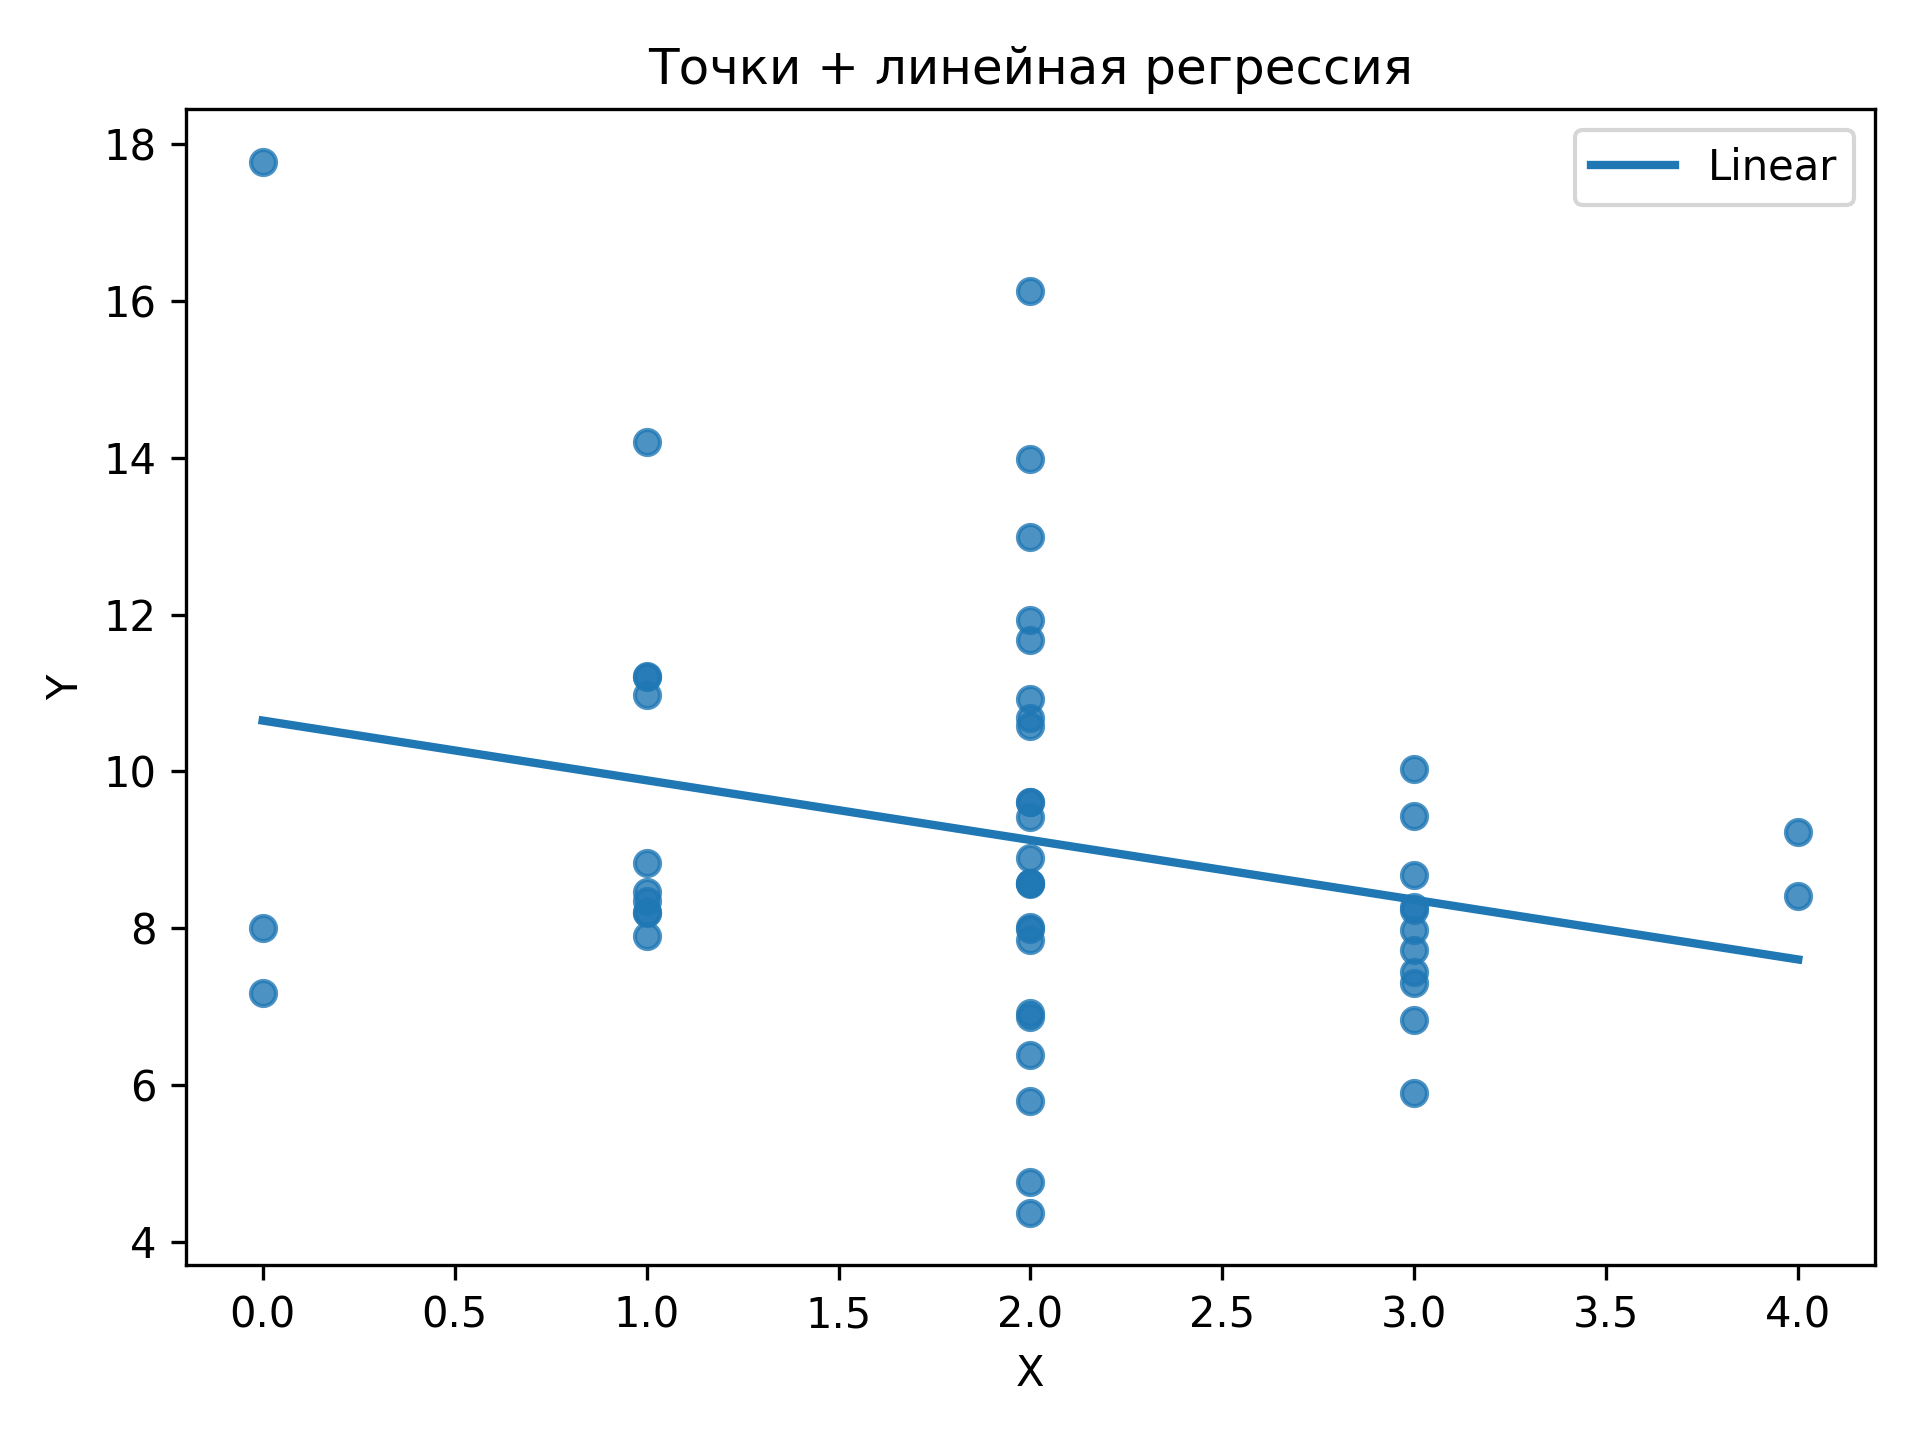
\includegraphics[width=.55\textwidth]{figs/task1_linear.png}
  \caption{Точки и линейная регрессия}
\end{figure}

%---------------------------------------------------------------
\subsection{Квадратичная модель}
\[
y_i=\beta_1+\beta_2x_i+\beta_3x_i^2+\varepsilon_i.
\]

\paragraph{Оценки МНК.}
Из $(X^\top X)^{-1}X^\top y$:
\[
\hat\beta_1=11.004,\;
\hat\beta_2=-1.238,\;
\hat\beta_3=0.124.
\]

\paragraph{Сумма квадратов остатков.}
\[
RSS_{\text{quad}}=309.92,\qquad
R^2_{\text{quad}}=0.074.
\]

\paragraph{AIC.}
$k=3\Rightarrow$
\(
\text{AIC}=50\ln(6.598)+6 = 239.36.
\)

\begin{figure}[H]
  \centering
  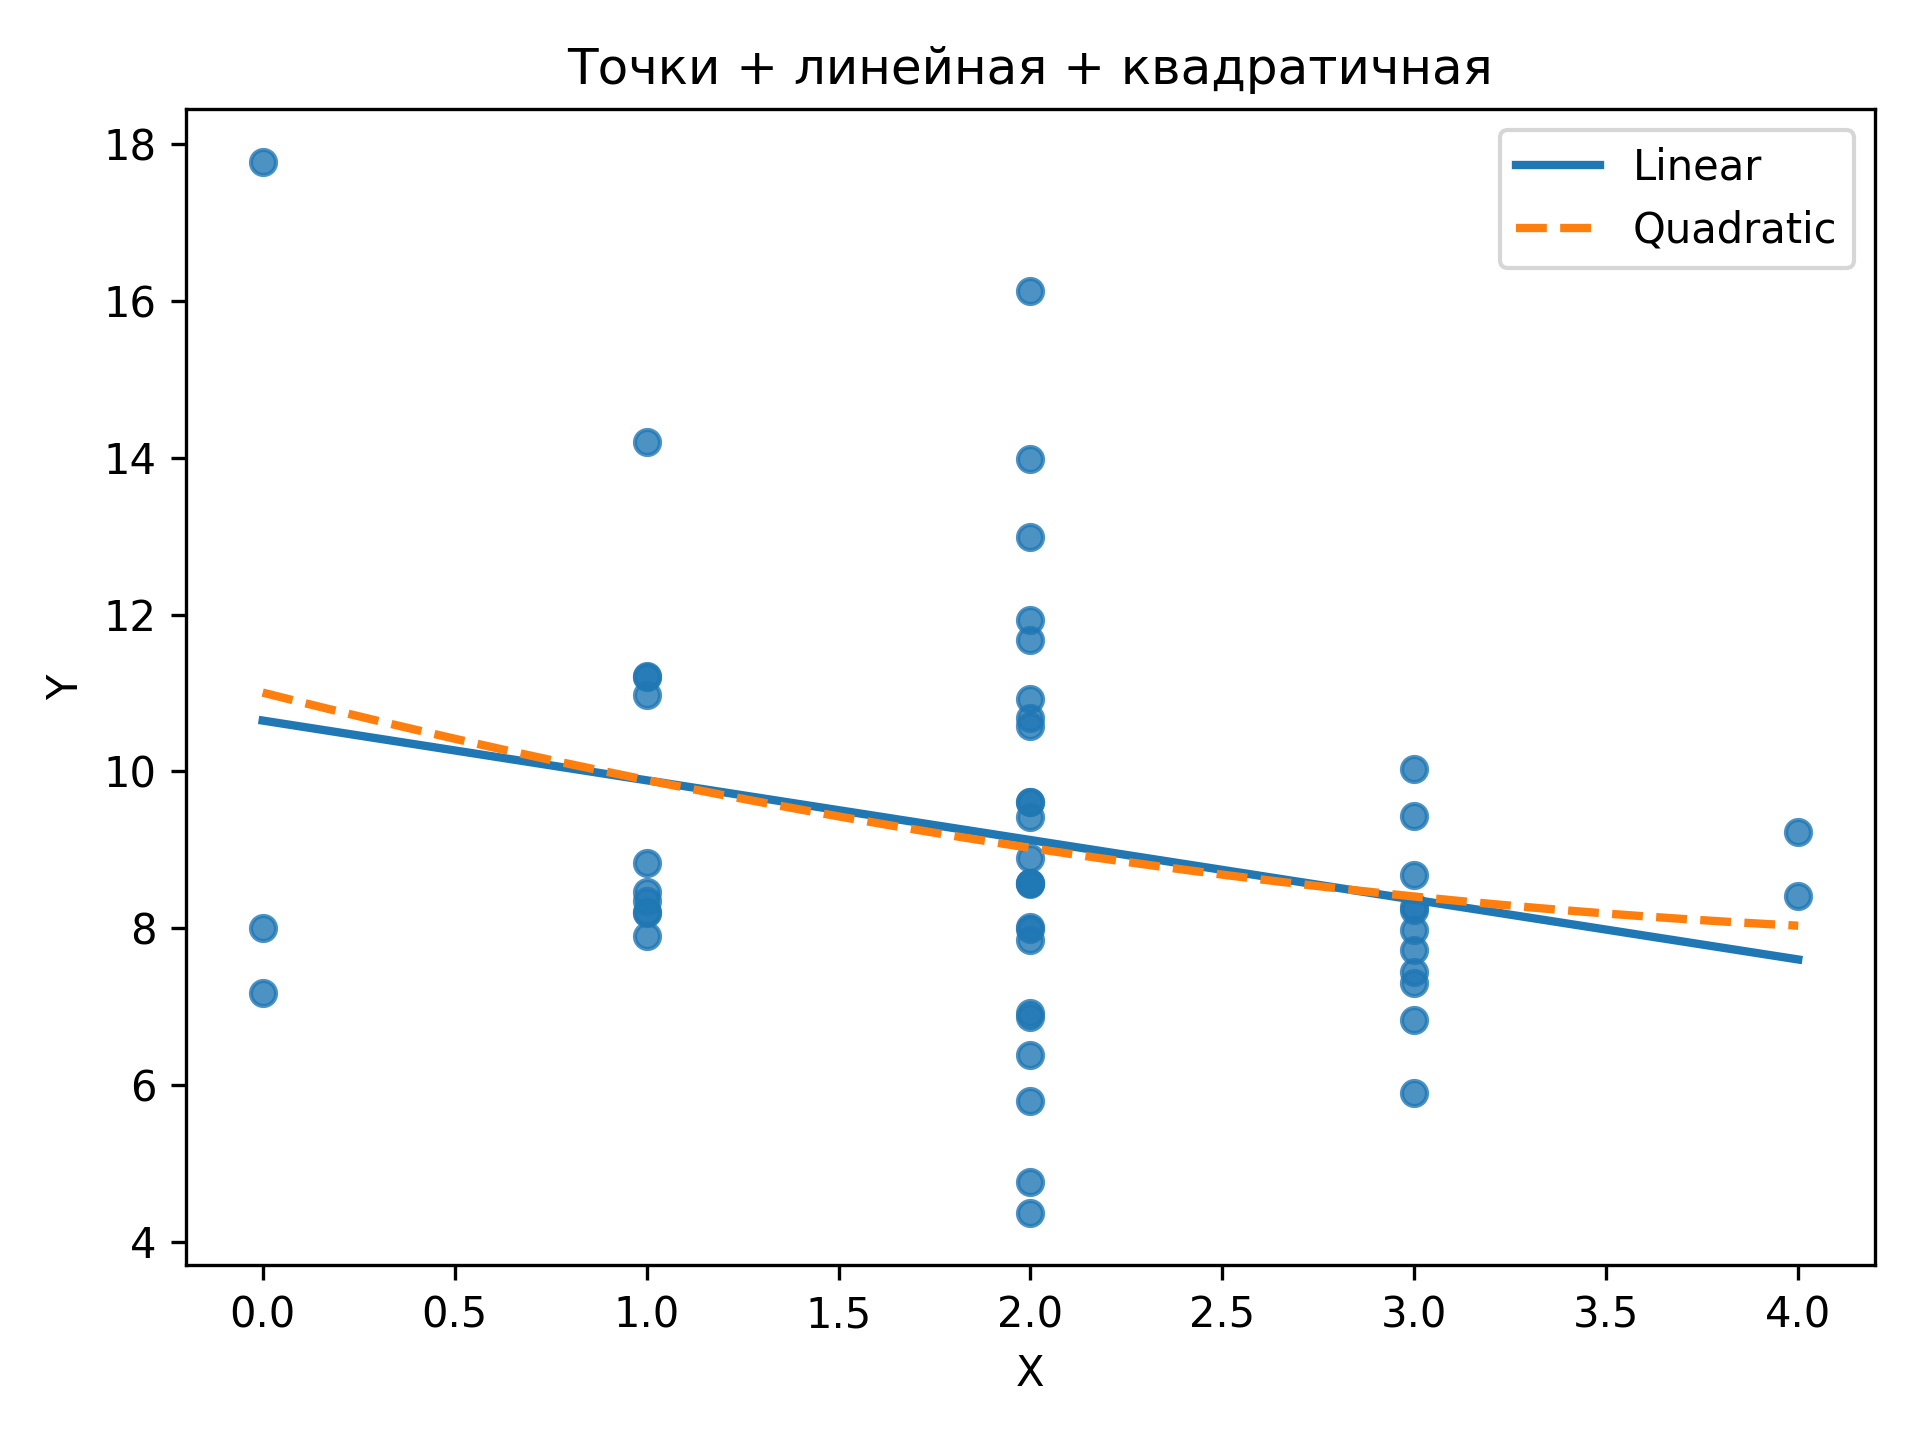
\includegraphics[width=.55\textwidth]{figs/task1_lin_quad.png}
  \caption{Линейная (сплошная) и квадратичная (штрих) регрессии}
\end{figure}

%---------------------------------------------------------------
\subsection{Доверительные интервалы (99 \%)}
\[
\hat\sigma^2=\frac{RSS_{\text{quad}}}{n-k}=6.603,\qquad
t_{0.995}(47)=2.69.
\]
\[
\operatorname{SE}(\hat\beta_2)=\sqrt{6.603\cdot0.0677}=0.669,\;
\operatorname{SE}(\hat\beta_3)=\sqrt{6.603\cdot0.0050}=0.181.
\]

\[
\beta_2:\;
\hat\beta_2\pm t\operatorname{SE}
 =-1.238\pm2.69\cdot0.669
 =\boxed{(-4.68;\,2.20)},
\]
\[
\beta_3:\;
\hat\beta_3\pm t\operatorname{SE}
 =0.124\pm2.69\cdot0.181
 =\boxed{(-0.72;\,0.97)}.
\]

%---------------------------------------------------------------
\subsection{Совместный доверительный эллипсоид (99 \%)}

Неравенство
\[
(\boldsymbol\beta-\hat{\boldsymbol\beta})^{\!\top}
(X^\top X)\,(\boldsymbol\beta-\hat{\boldsymbol\beta})
\le 2\hat\sigma^{2}\,F_{2,47}(0.99)=\boxed{67.43}
\]
задаёт эллипс в плоскости $(\beta_2,\beta_3)$.

Параметры эллипса  
\[
\hat\beta_2=-1.238,\qquad
\hat\beta_3= 0.124,\qquad
a=\sqrt{c\,\lambda_{\max}},\;
b=\sqrt{c\,\lambda_{\min}},\;
c=2F_{2,47}(0.99),
\]
где $\lambda_{\max},\lambda_{\min}$ — собственные значения матрицы
$\hat\sigma^{2}(X^\top X)^{-1}$.

\begin{figure}[H]
  \centering
  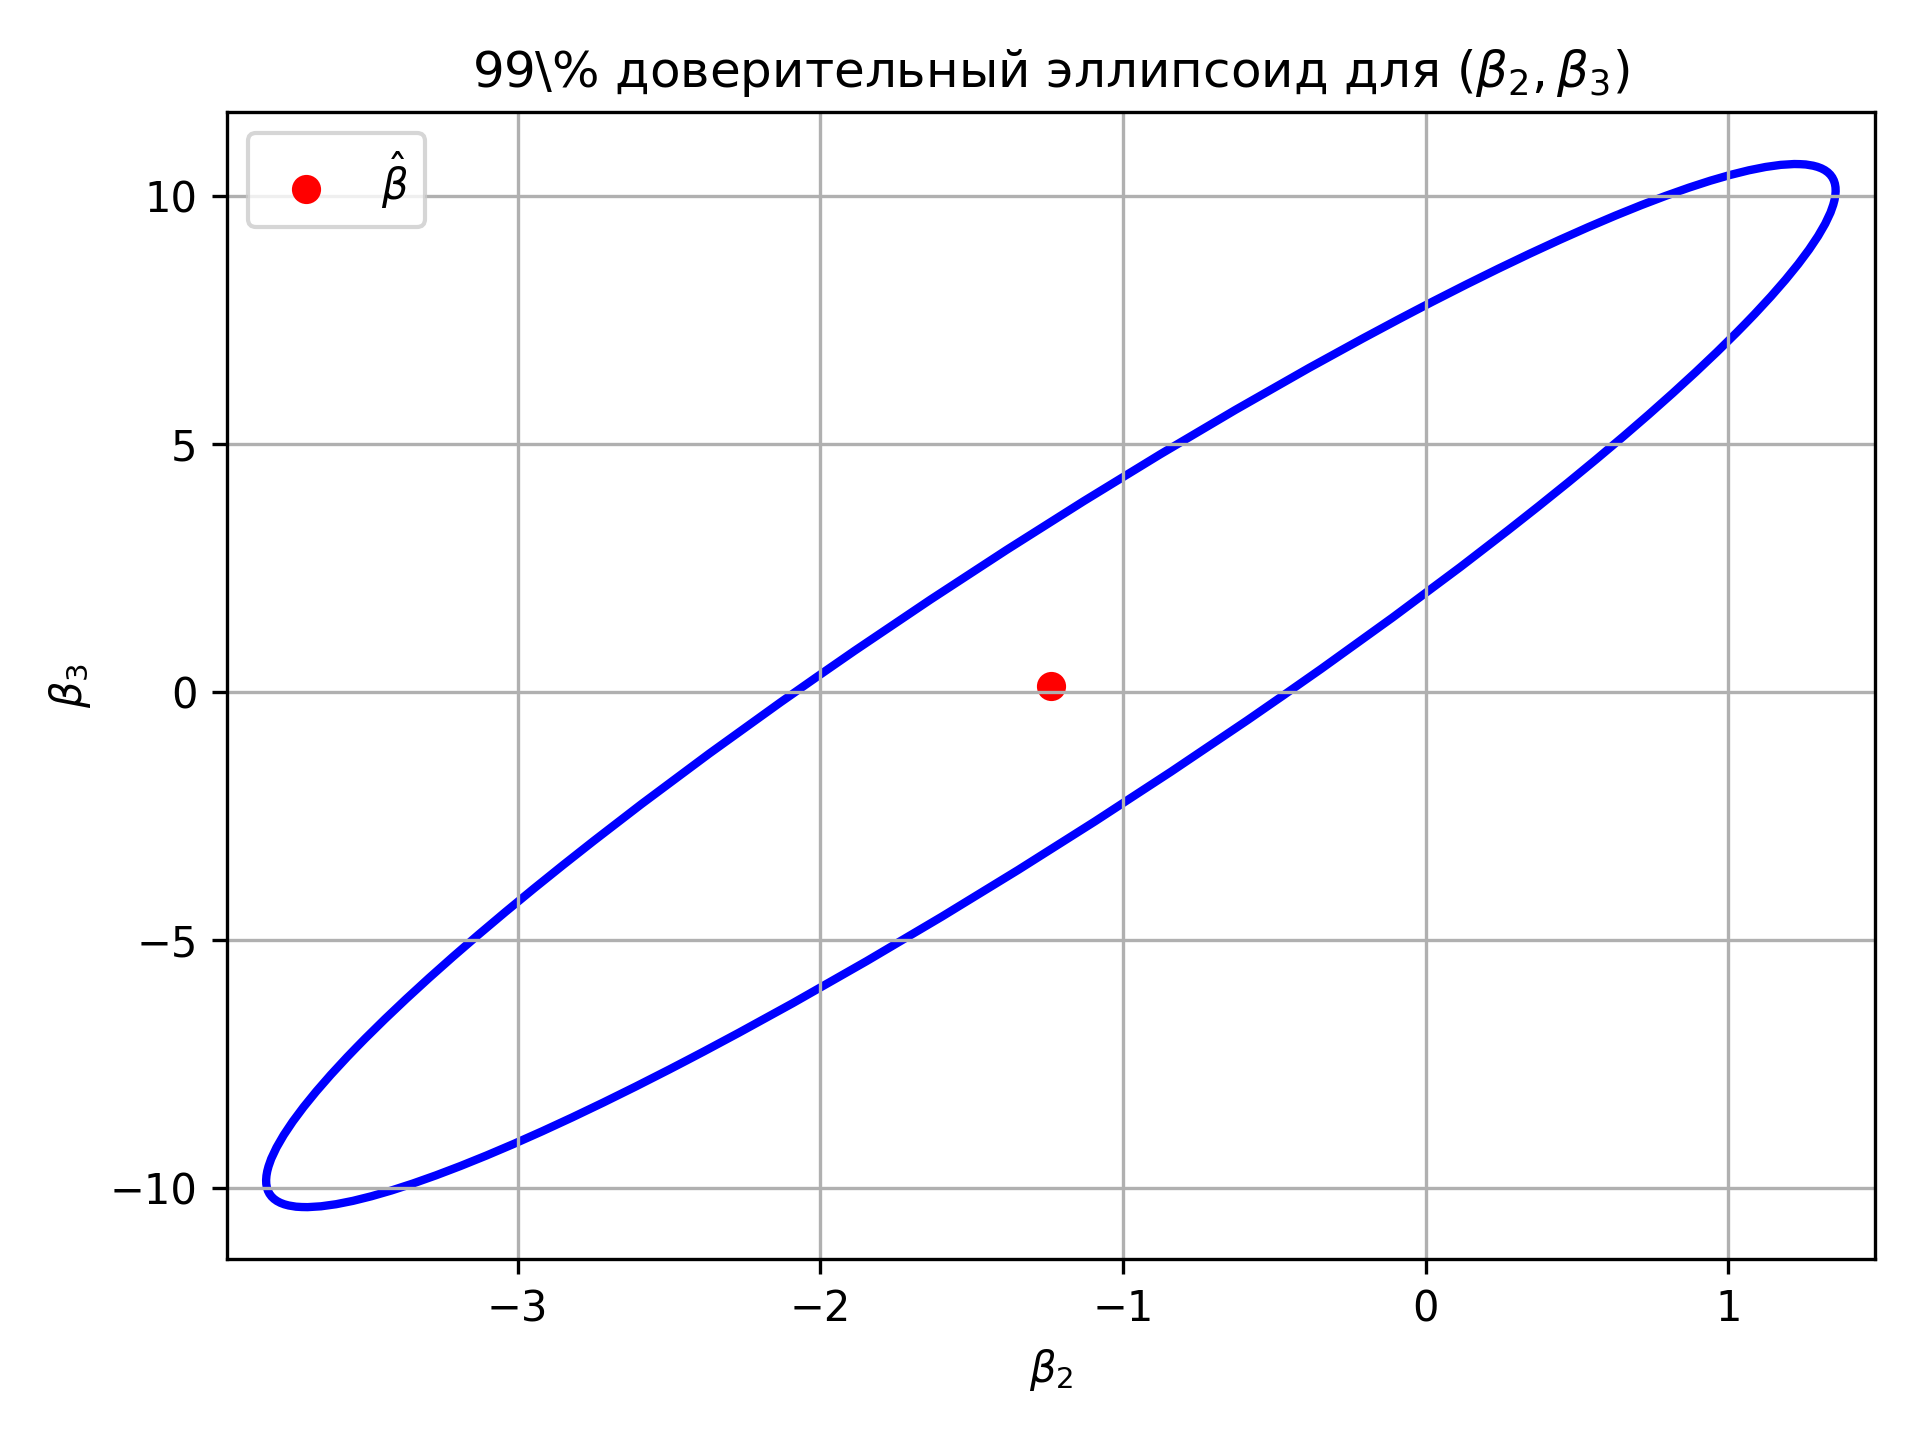
\includegraphics[width=.55\textwidth]{figs/task1_conf_ellipse.png}
  \caption{99-\% доверительный эллипсоид для параметров $\beta_2,\beta_3$}
\end{figure}


%---------------------------------------------------------------
\subsection{Проверка гипотез}
\paragraph{Линейность ($H_0:\beta_3=0$).}
\[
F=\frac{RSS_{\text{lin}}-RSS_{\text{quad}}}{1}\Big/
  \frac{RSS_{\text{quad}}}{n-3}
  =0.153,\; p=0.697>0.01\;\Rightarrow\;H_0\text{ не отвергается.}
\]

\paragraph{Независимость ($H_0:\beta_2=0$).}
\[
t=\frac{\hat\beta_2}{\operatorname{SE}(\hat\beta_2)}
  =-1.912,\; p=0.062>0.01\;\Rightarrow\;H_0\text{ не отвергается.}
\]

%---------------------------------------------------------------
\subsection{Анализ остатков}
\[
\chi^2=\sum_{j=1}^{m}
\frac{(O_j-E_j)^2}{E_j}=9.50,\;
p=0.091;
\qquad
JB=\frac{n}{6}(s^2+\tfrac14k^2)=6.72,\;
p=0.035.
\]

\begin{figure}[H]
  \centering
  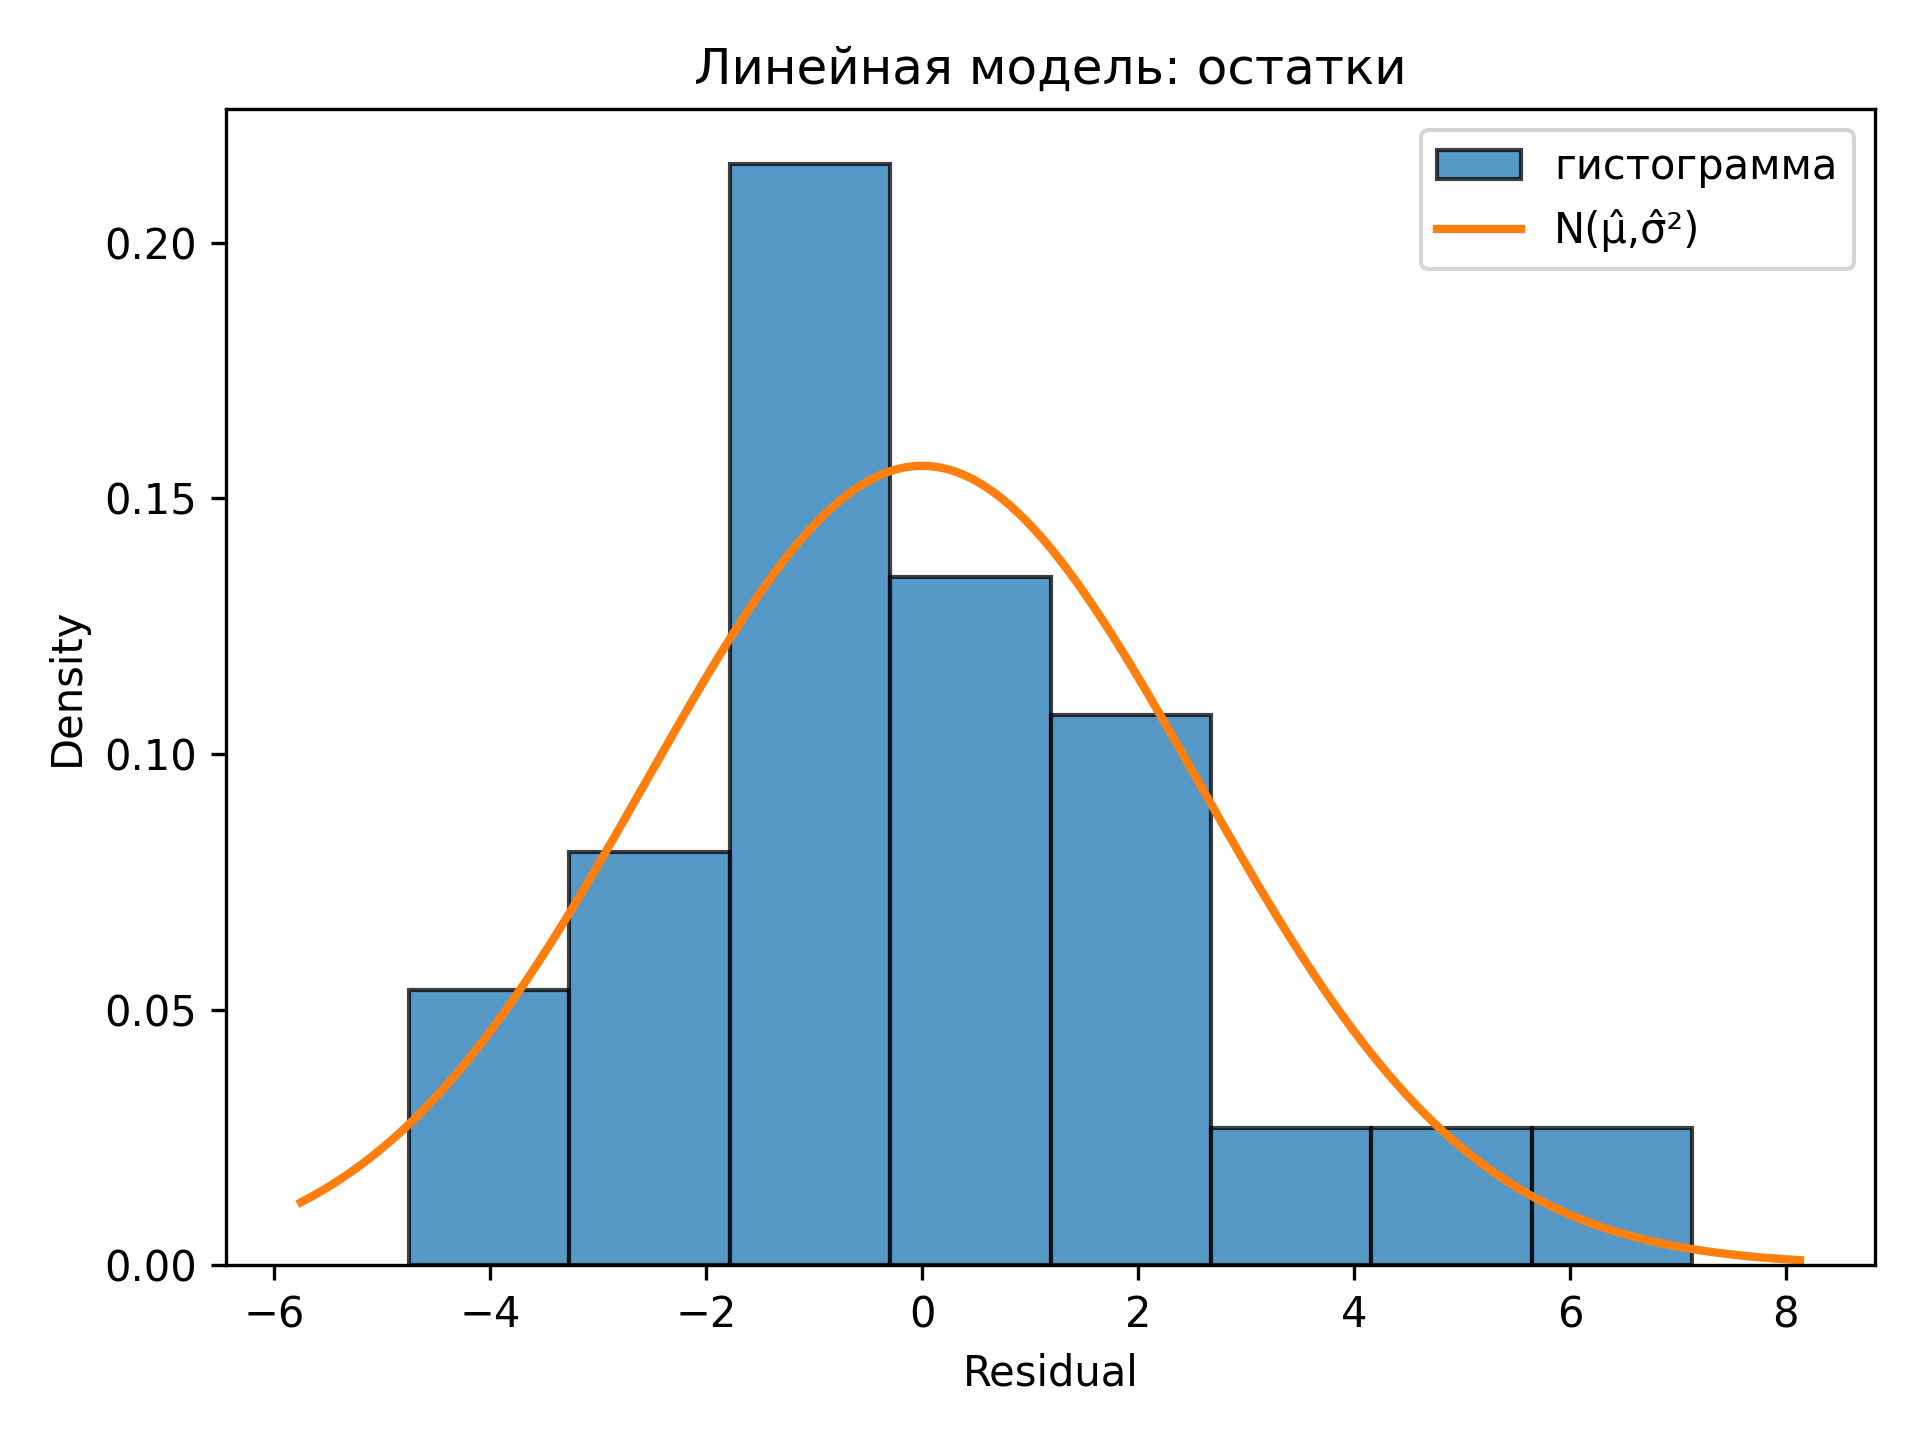
\includegraphics[width=.48\textwidth]{figs/task1_resid_hist_lin.png}\hfill
  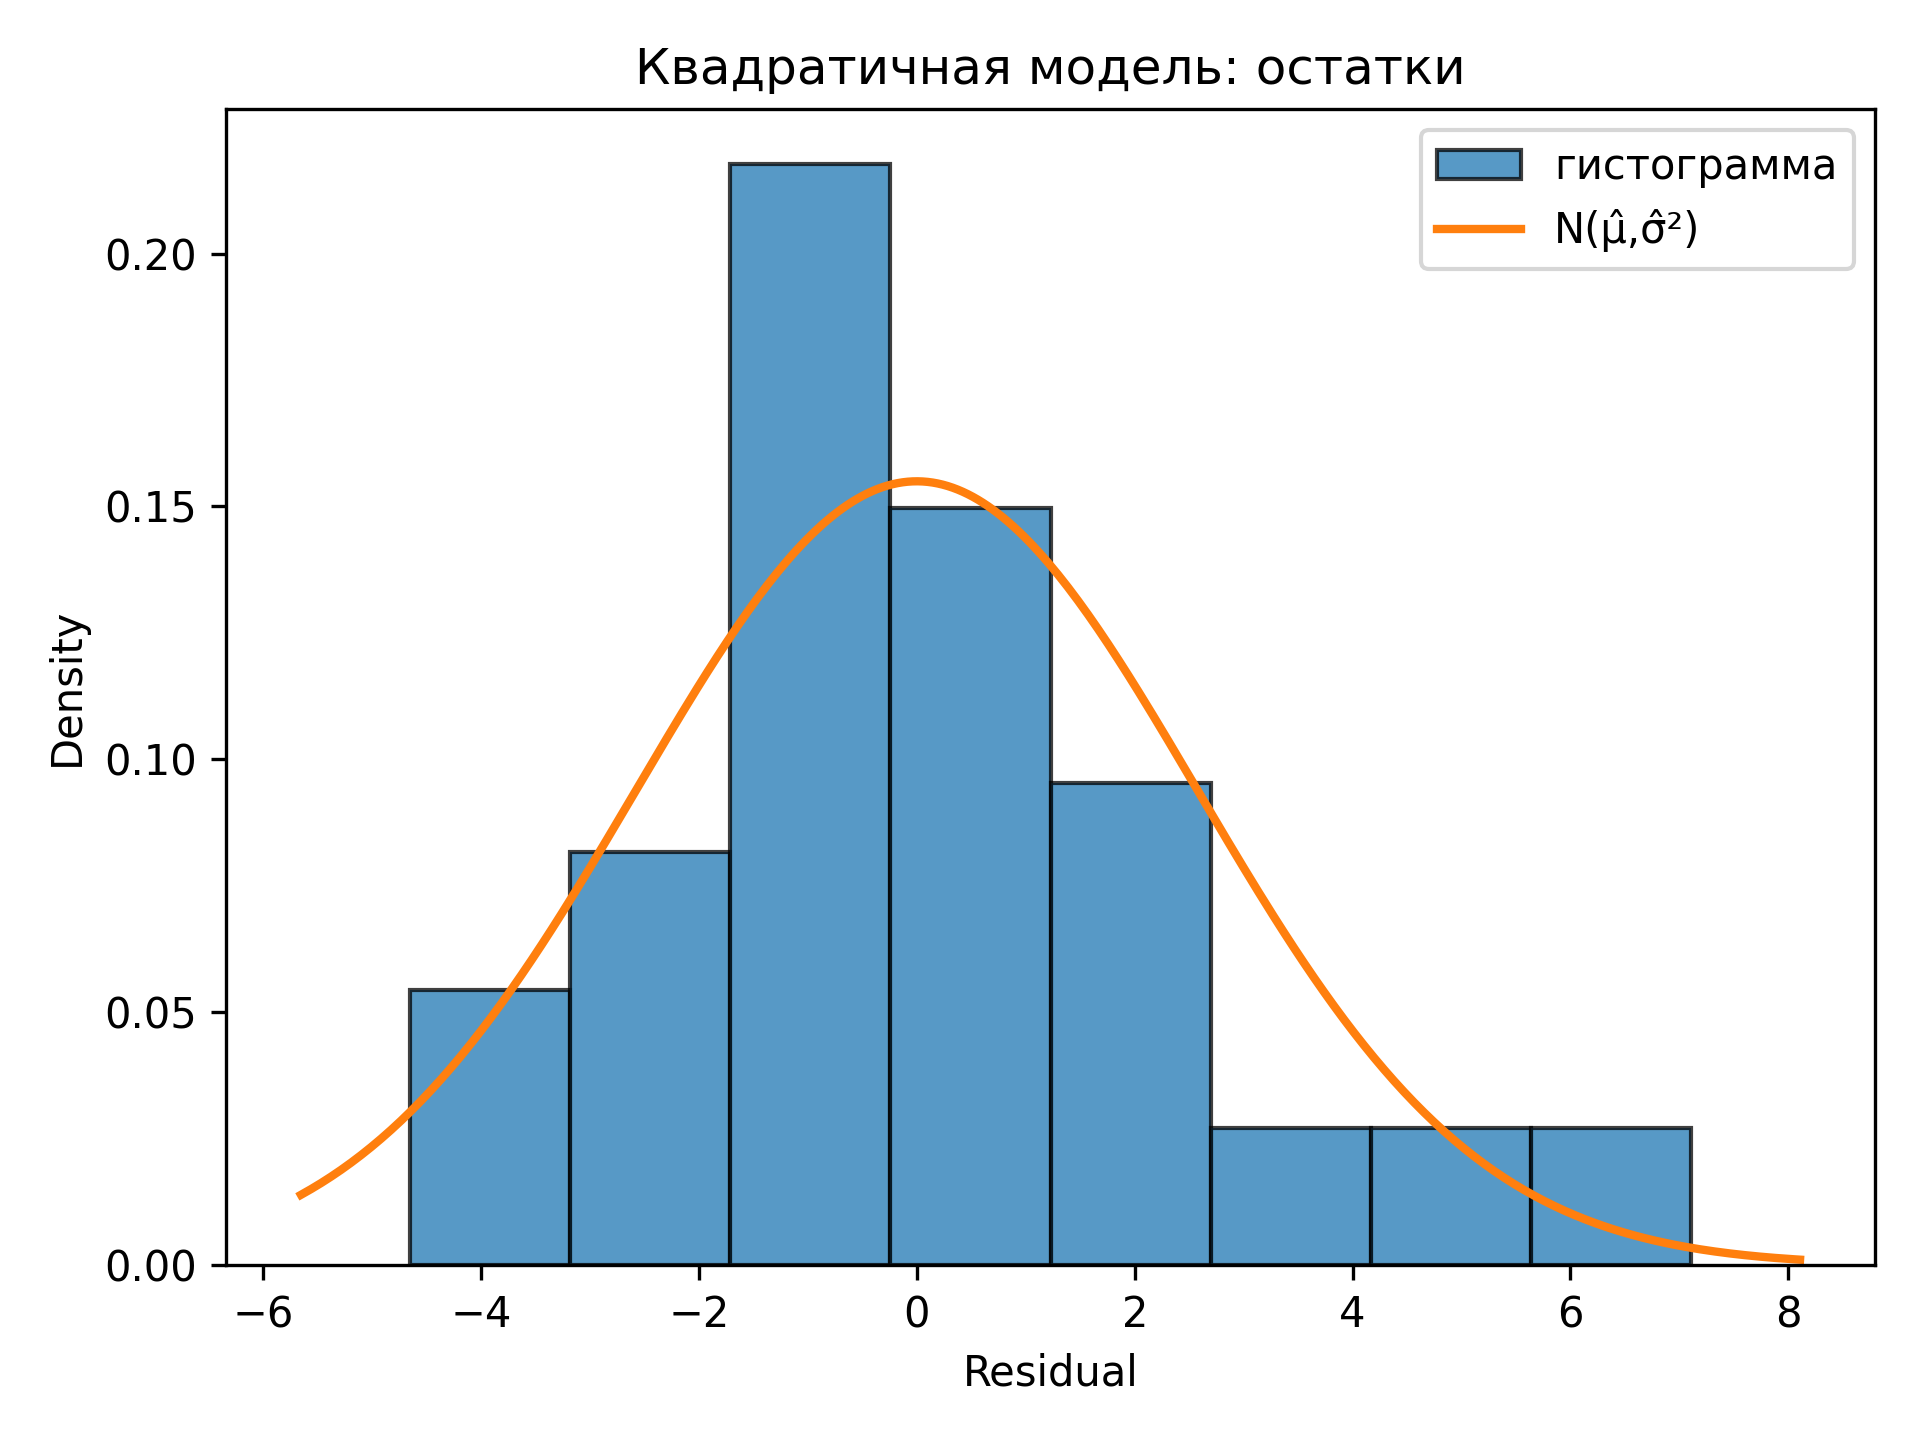
\includegraphics[width=.48\textwidth]{figs/task1_resid_hist_poly.png}
  \caption{Остатки линейной (слева) и квадратичной (справа) моделей}
\end{figure}

%---------------------------------------------------------------
\subsection{Итог задачи 1}
$\Delta\text{AIC}=1.84<2$ → линейная и квадратичная модели одинаково
информативны; выбираем более простую.  
При этом $R^2\!\approx\!7\%$ — переменная $X$ объясняет лишь малую часть
дисперсии~$Y$.

%=================================================================
\section{Задача 2 — влияние факторов $A$ и $B$}
\subsection{Статистическая модель}
\[
y_{ijk}= \mu+\alpha_i+\beta_j+(\alpha\beta)_{ij}+\varepsilon_{ijk},
\quad
\varepsilon_{ijk}\sim N(0,\sigma^2),
\]
\[
i=1,\dots,4,\; j=1,\dots,4,\; k=1,\dots,n_{ij},\;
\sum_i\alpha_i=\sum_j\beta_j=\sum_i(\alpha\beta)_{ij}
               =\sum_j(\alpha\beta)_{ij}=0.
\]

%---------------------------------------------------------------
%---------------------------------------------------------------
\subsection{F-тесты для факторов и взаимодействия}
\[
F_H=\frac{MS_H}{MS_E},\qquad
MS_H=\frac{SS_H}{df_H},\;
MS_E=\frac{SS_E}{df_E},\;
H\in\{A,B,AB\}.
\]

\begin{table}[H]\centering
  \caption{F-тесты для факторов и взаимодействия}
\begin{tabular}{l|ccccc}
  \toprule
  Источник $H$ & $SS_H$ & $df_H$ & $MS_H$ & $MS_E$ & $F_H$\\
  \midrule
  $A$         & 979.34 & 3 & 326.45 & 2.76 & \textbf{118.30}\\
  $B$         & 513.23 & 3 & 171.08 & 2.76 & \textbf{61.99}\\
  $A\times B$ & 1047.67& 9 & 116.41 & 2.76 & \textbf{42.18}\\
  \bottomrule
  \end{tabular}
  \end{table}
  Критические значения: \(F_{3,32}^{0.99}=4.01,\;
  F_{9,32}^{0.99}=3.04\).
  Поскольку все наблюдаемые \(F_H\) $\gg$ \(F_{crit}\),
  отвергаем нулевые гипотезы об отсутствии эффекта
  как факторов \(A,B\), так и их взаимодействия \(A\times B\)
  (уровень значимости \(1\%\)):
  
  \[
  p_A<10^{-15},\qquad
  p_B<10^{-12},\qquad
  p_{AB}=3\cdot10^{-15}.
  \]

%---------------------------------------------------------------
\subsection{Информационные критерии}
\begin{table}[H]\centering
  \caption{Информационные критерии моделей}
  \begin{tabular}{l|ccccc}
  \toprule
  Модель & $k$ & $\hat\sigma^{2}$ & AIC & BIC\\
  \midrule
  $A*B$ & 16 & 2.76  & 197.5 & 227.4\\
  $A+B$ &  7 & 10.45 & 302.1 & 315.2\\
  $A$   &  4 & 21.66 & 314.0 & 321.5\\
  \bottomrule
  \end{tabular}
  \end{table}
  

%---------------------------------------------------------------

\subsection{Визуальное взаимодействие}
\begin{figure}[H]
  \centering
  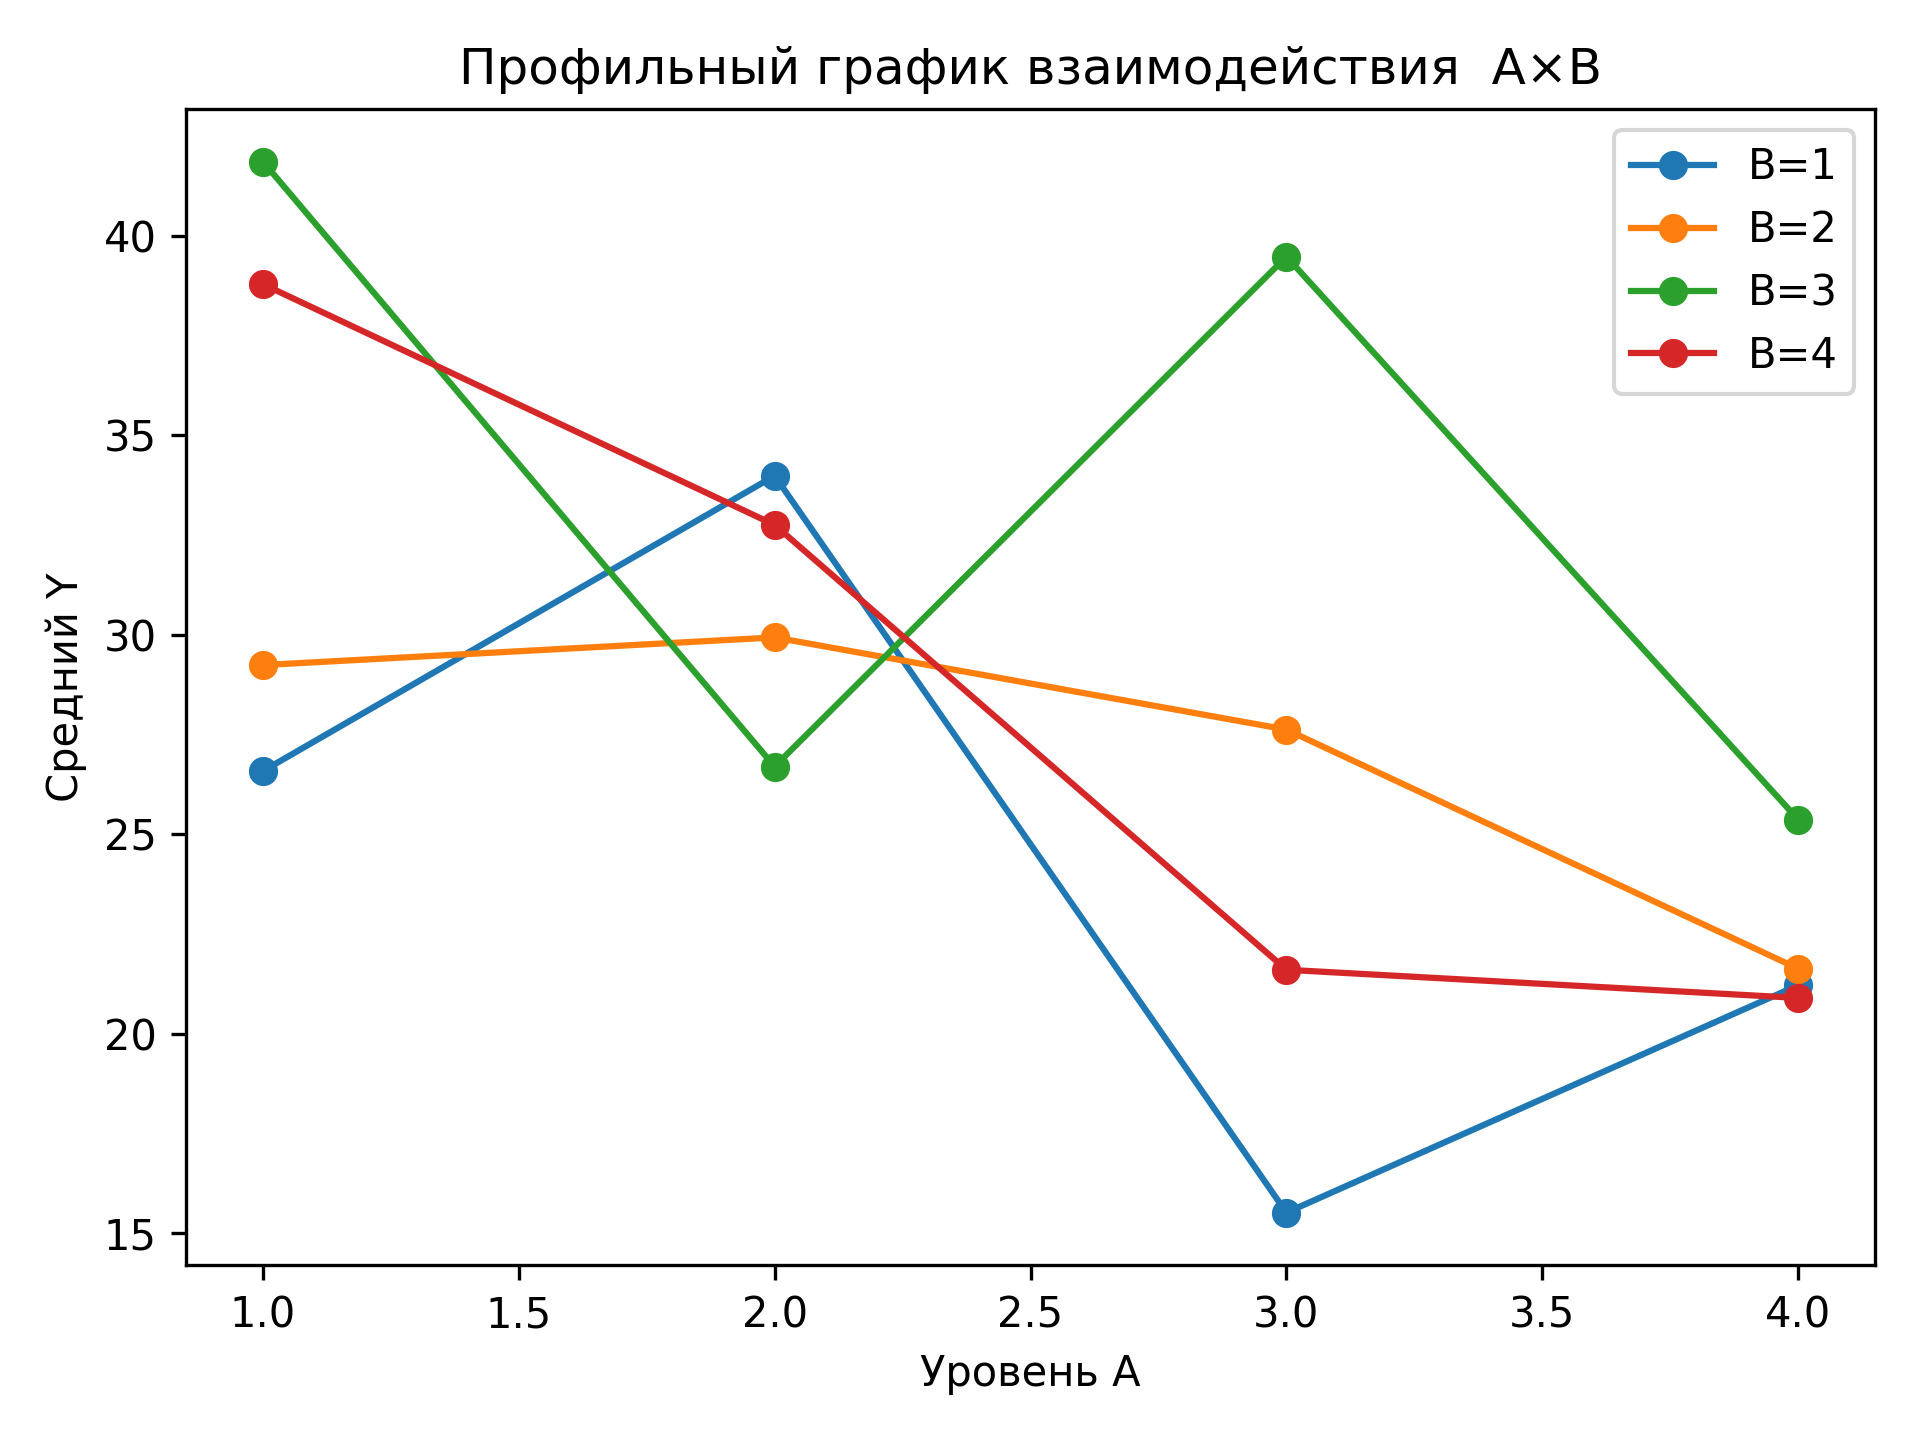
\includegraphics[width=.6\textwidth]{figs/task2_interaction.png}
  \caption{Профильные графики: средние $Y$ при разных $B$}
\end{figure}

%---------------------------------------------------------------
\subsection{Разложение сумм квадратов}
\[
\begin{aligned}
SS_{\text{T}}&=\sum_{i,j,k}(y_{ijk}-\bar y_{\cdot\cdot\cdot})^2,\\
SS_A&=\sum_i n_{i\cdot}(\bar y_{i\cdot\cdot}-\bar y_{\cdot\cdot\cdot})^2
      =979.34,\\
SS_B&=\sum_j n_{\cdot j}(\bar y_{\cdot j\cdot}-\bar y_{\cdot\cdot\cdot})^2
      =513.23,\\
SS_{AB}&=\sum_{i,j} n_{ij}(\bar y_{ij\cdot}-\bar y_{i\cdot\cdot}
          -\bar y_{\cdot j\cdot}+\bar y_{\cdot\cdot\cdot})^2
        =1047.67,\\
SS_E&=SS_{\text{T}}-SS_A-SS_B-SS_{AB}=88.30.
\end{aligned}
\]

\[
\begin{array}{l|cccc}
\text{Источник} & SS & df & MS & F\\\hline
A & 979.34 & 3 & 326.45 & 326.45/2.76 =118.3\\
B & 513.23 & 3 & 171.08 & 171.08/2.76 = 62.0\\
AB&1047.67 & 9 & 116.41 & 116.41/2.76 = 42.18\\
E &  88.30 &32 & 2.76 & \\
\end{array}
\]

%---------------------------------------------------------------
\subsection{Проверка взаимодействия}
\[
F_{AB}=\frac{MS_{AB}}{MS_E}=42.18,\quad
p=3\cdot10^{-15}\ll0.01.
\]

%---------------------------------------------------------------
\subsection{Анализ остатков}
Jarque–Bera для полной модели:
\[
JB=\frac{n}{6}\bigl(s^2+\tfrac14k^2\bigr)=1.10,\quad p=0.576.
\]

\begin{figure}[H]
  \centering
  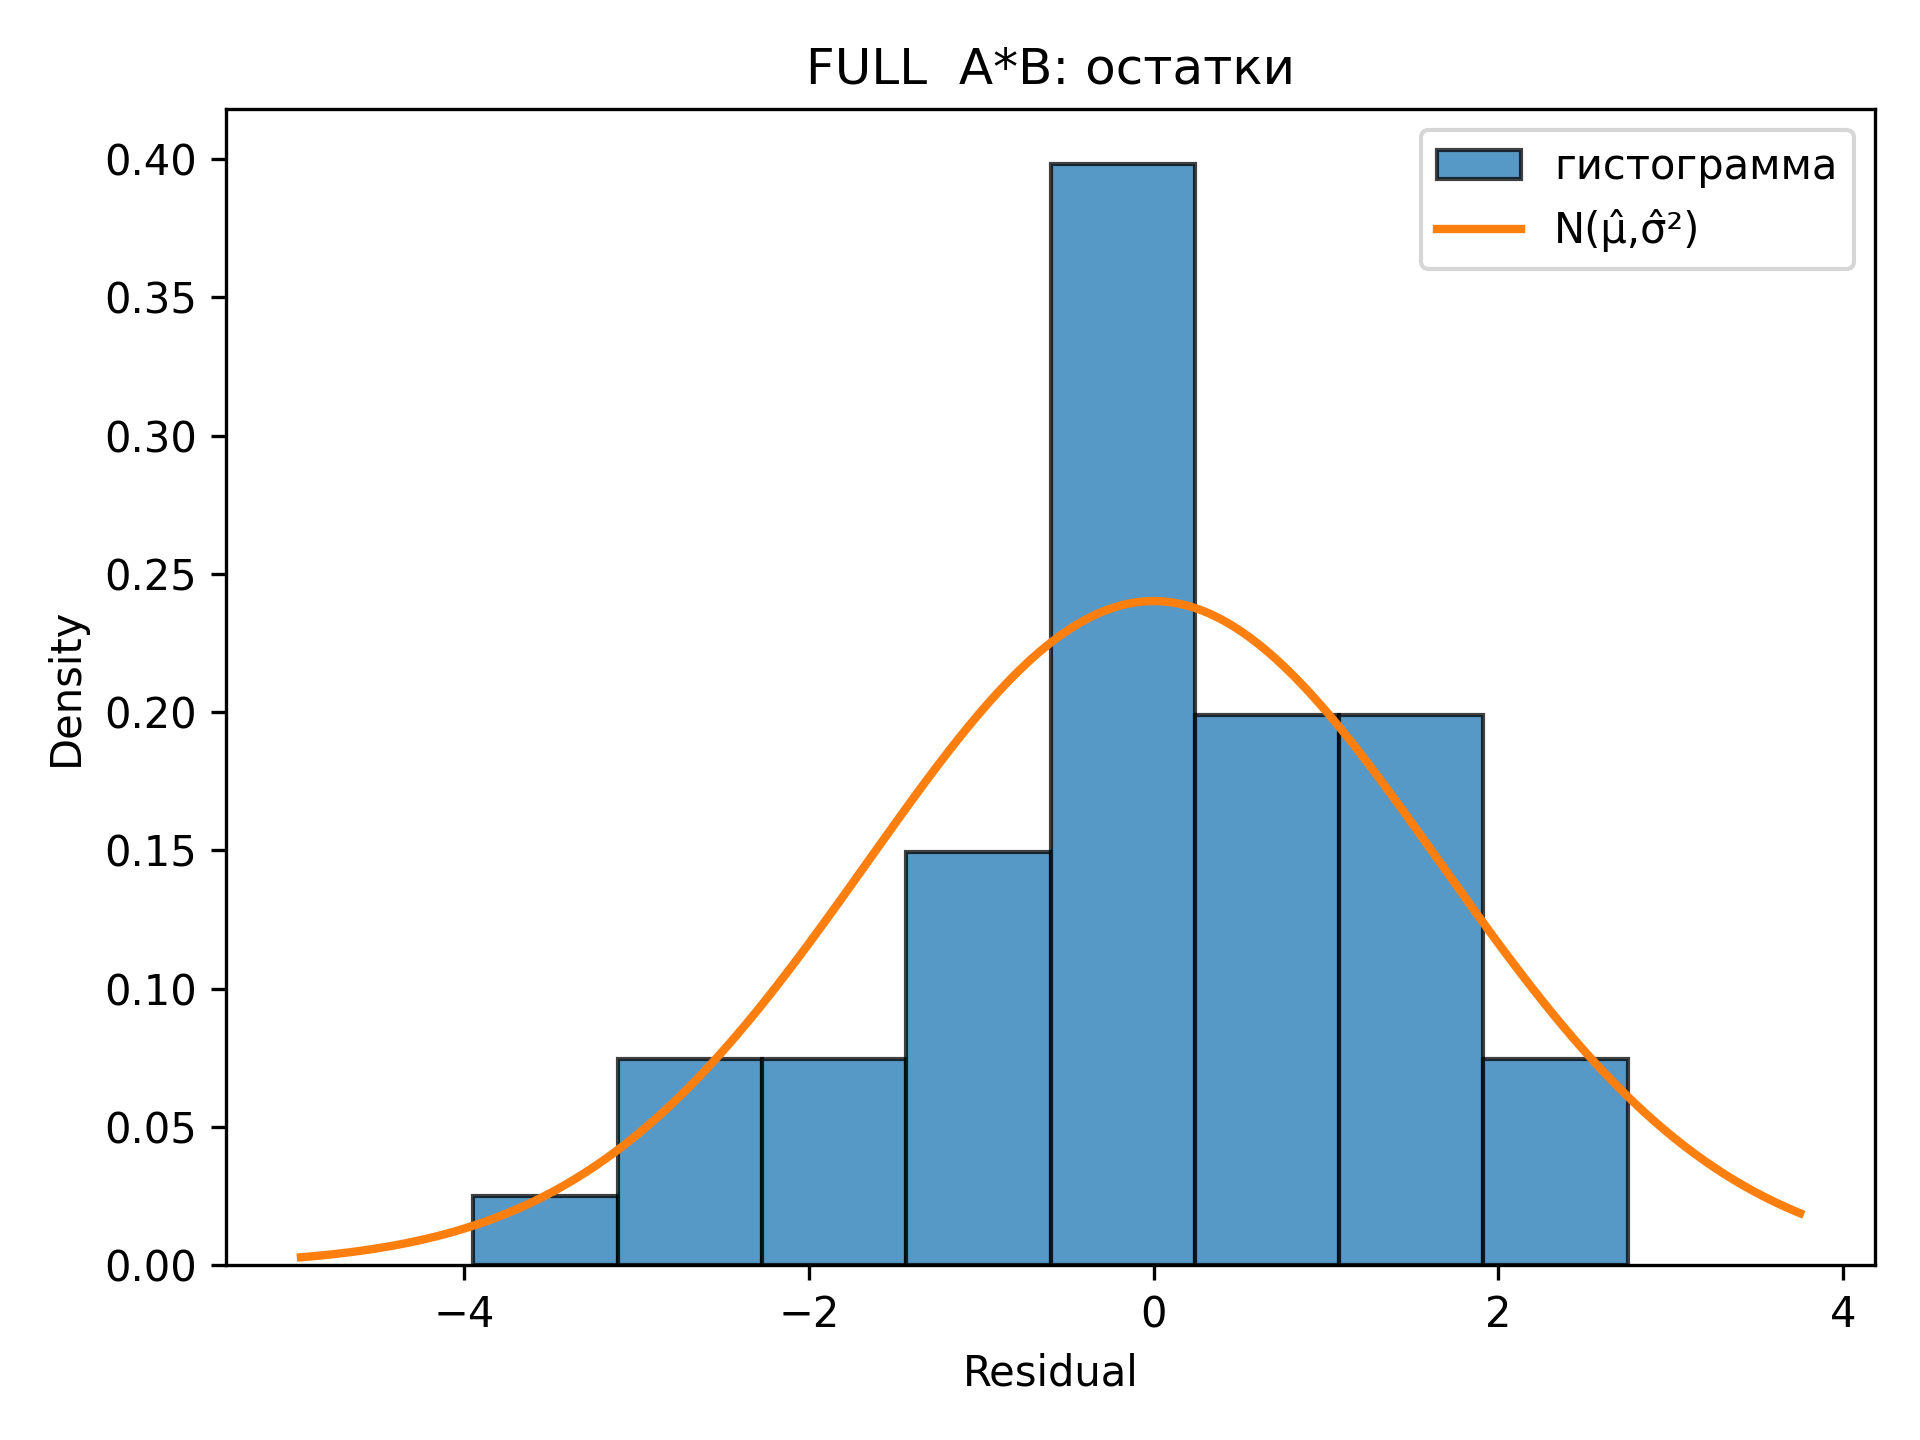
\includegraphics[width=.48\textwidth]{figs/task2_resid_hist_full.png}\hfill
  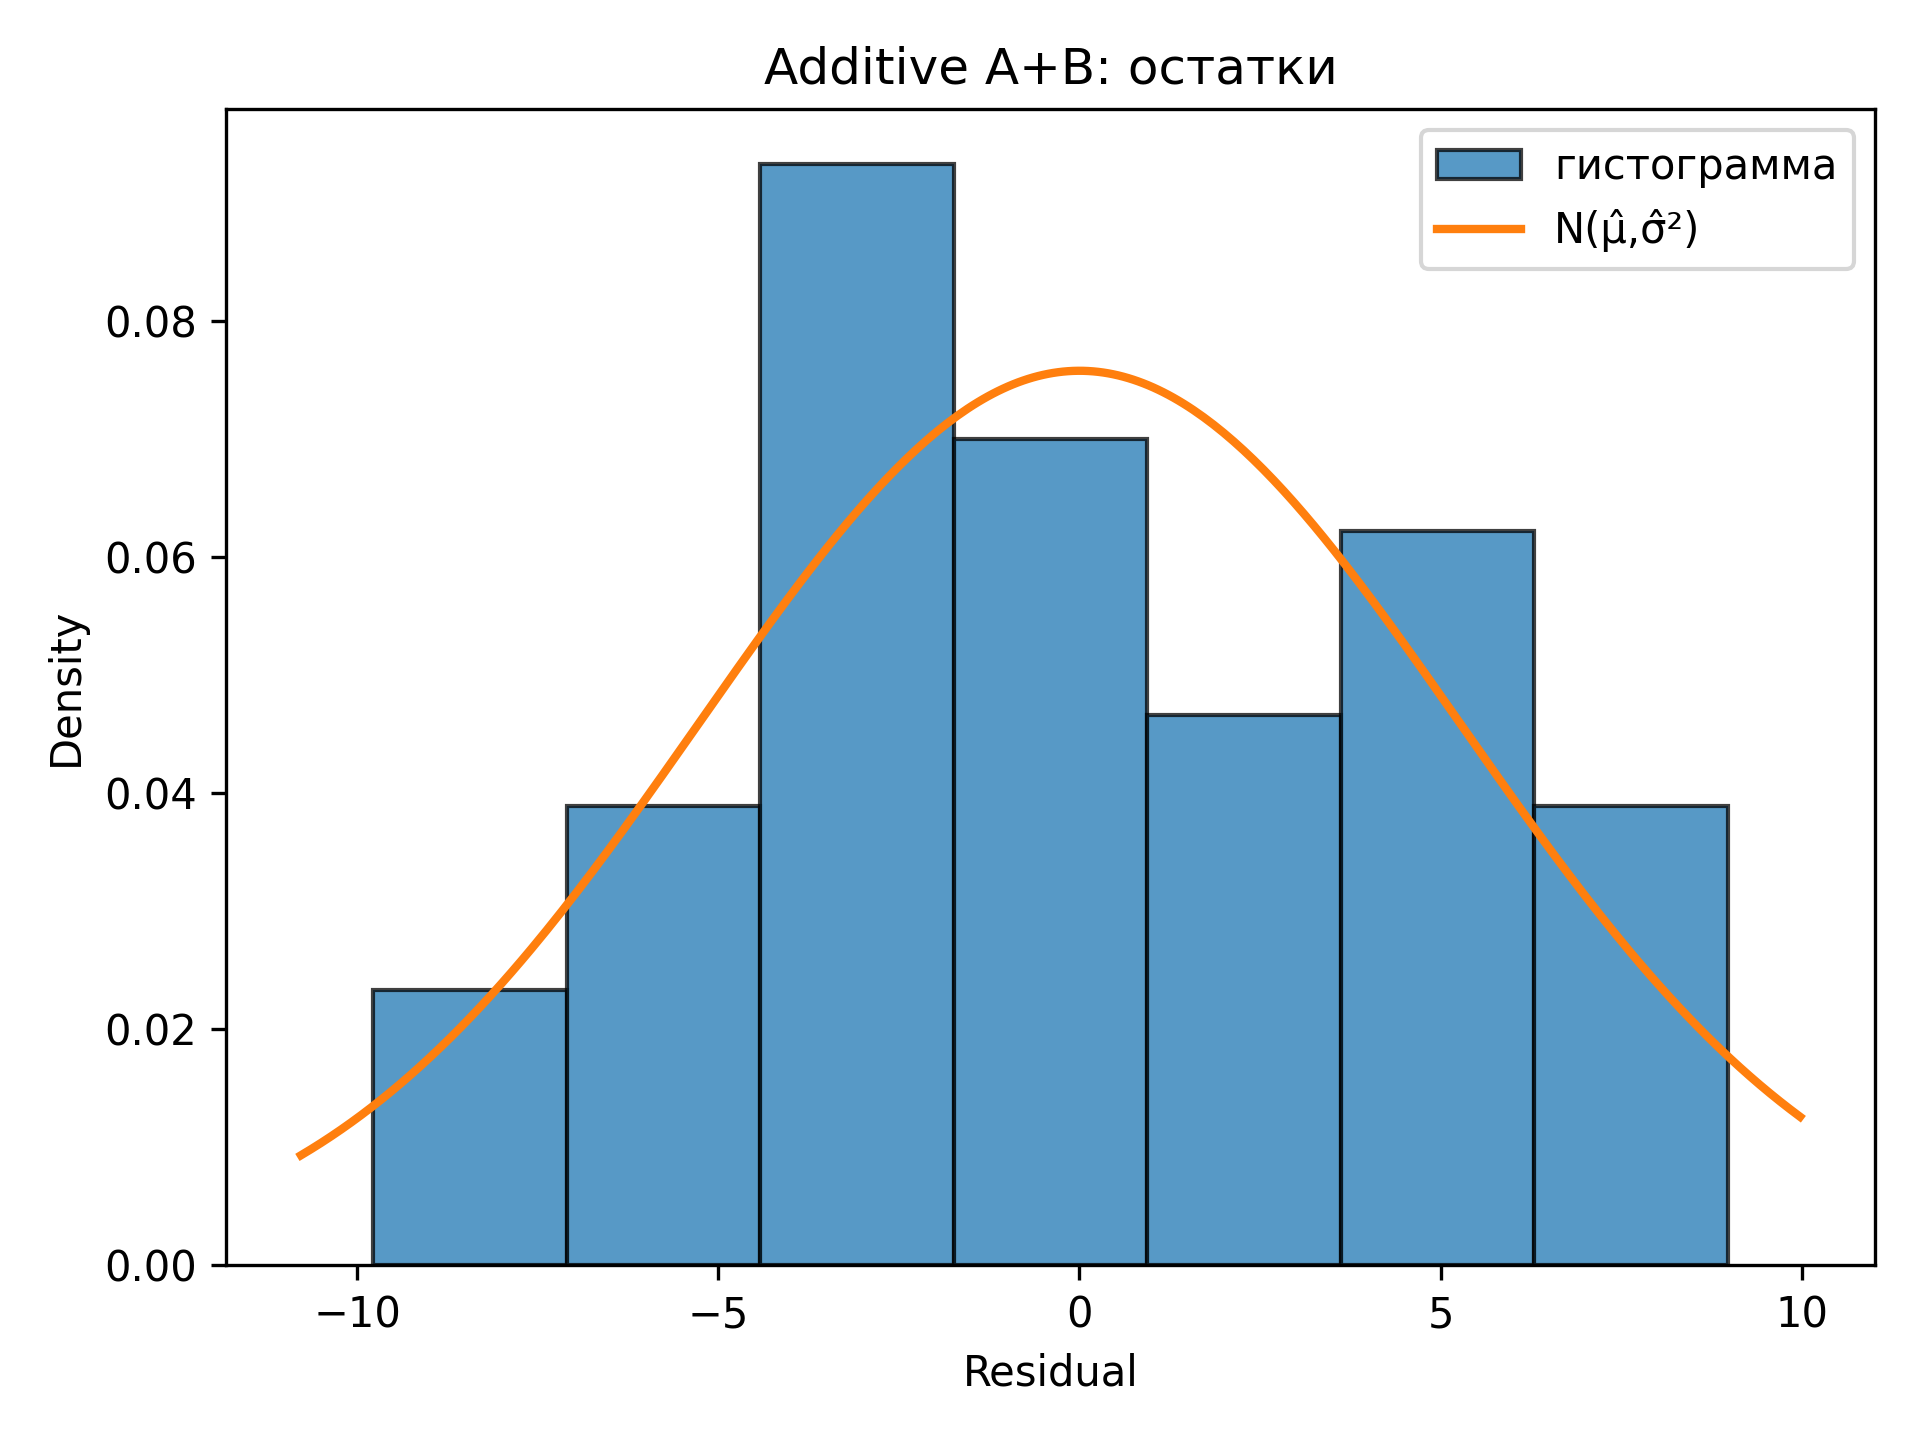
\includegraphics[width=.48\textwidth]{figs/task2_resid_hist_add.png}
  \caption{Гистограммы остатков полной (слева) и аддитивной (справа) моделей}
\end{figure}

%---------------------------------------------------------------
\subsection{Итог задачи 2}
\begin{itemize}[nosep]
  \item Значимы главные эффекты $A$, $B$ и взаимодействие $A\times B$  
        ($p<10^{-12}$).
  \item Лучшая по AIC/BIC модель: $Y\sim A*B$.
  \item Остатки нормальны, $\hat\sigma^2=2.76$.
\end{itemize}

\newpage
%=================================================================
\section*{Заключение}
\addcontentsline{toc}{section}{Заключение}
В задаче 1 слабая и статистически незначимая зависимость $Y$ от $X$,
при $R^2\approx7\%$ достаточно линейной модели.  
В задаче 2 найдено сильное влияние как каждого фактора, так и их
взаимодействия; выбрана полная модель $A*B$.
\[ F_crit = F_{\alpha, df_H, df_E} = \frac{1}{B(\frac{df_H}{2}, \frac{df_E}{2})} \int_{0}^{\frac{df_H}{df_H + df_E x}} t^{\frac{df_H}{2}-1} (1-t)^{\frac{df_E}{2}-1} dt \]


В 13 определении -> компактно записать задачи 
\[ 
H_0: a=a_0
T = \sqrt(n-1) \frac{\hat{x}-a}{s}
T~S_{n-1}
\phi(x) = \begin{cases}
  0, & T \in [-x_\alpha, x_\alpha] \\
  1, & x \notin [-x_\alpha, x_\alpha]
  \end{cases}
x_\alpha = {S^{-1}}_n-1 (1-\alpha/2)
\]
\end{document}